\documentclass{article}
\usepackage{graphicx}
\usepackage{listings}
\usepackage{color}
\usepackage{listings}
\usepackage{multicol}
\usepackage{courier}
\usepackage{subcaption}
\graphicspath{ {Images/} }

\topmargin0.0cm
\headheight0.0cm
\headsep0.0cm
\oddsidemargin0.0cm
\textheight23.0cm
\textwidth16.5cm
\footskip1.0cm

\definecolor{dkgreen}{rgb}{0,0.6,0}
\definecolor{gray}{rgb}{0.5,0.5,0.5}
\definecolor{mauve}{rgb}{0.58,0,0.82}

\lstset{frame=tb,
  aboveskip=3mm,
  belowskip=3mm,
  showstringspaces=false,
  basicstyle={\small\ttfamily},
  numbers=none,
  numberstyle=\tiny\color{gray},
  keywordstyle=\color{blue},
  commentstyle=\color{dkgreen},
  stringstyle=\color{mauve},
  breaklines=true,
  breakatwhitespace=true,
  tabsize=2
}

\makeatletter
\def\and{%
  \end{tabular}%
  \hskip 0.0001em \@plus.17fil\relax
  \begin{tabular}[t]{c}}

\setlength\parindent{0pt} % Removes all indentation from paragraphs

\begin{document}

\title{\textbf{WACC 20: Reflection and Extension} \\ Imperial College London \\ Autumn}
\author{
  Paul Li\'etar\\
  \texttt{pl2113}
  \and
  Leanne Lyons\\
  \texttt{ll5914}
  \and
  Jaime Rodr\'iguez\\
  \texttt{jr1314}
  \and
  Ignacio Navarro\\
  \texttt{in714}
}
\date{}

\maketitle

\section{Product}
Analysis and critical evaluation of the quality of WACC.
Our WACC compiler has been written in Haskell. This has allowed us to use powerful pattern matching and monads to write our compiler. Being extremely critical, we think we have built a fantastic compiler; it passes all the test cases, it has some great extensions and most importantly it does it fundamental job of preserving the meaning of the program being compiled whilst converting it into WACC.

The layout of our WACC compiler is very clear and concise, within our source folder you can easily see what is required for the Frontend, the Backend and the extension. Each file has one meaningful purpose e.g. our Parser.hs parses input, our SemCheck.hs carries out semantic checking. 

The fact that our compiler is well formatted means that it is quite easily extendible if you wanted to add to the WACC language. Adding additional statements would not cause any conflicts with the existing program; all you need to do is add it to the parser, add the correct semantic check and then add how you want the code to be generated using the IR (Intermediate Representation) we have already defined. 

We changed the register allocation in our extension to produce better code. This, however, means that our final register allocation is a bit slower than what we initially committed for the backend. This slowdown actually causes LabTS to timeout on one of our test cases so this is definitely something we would need to address if rebuilding the compiler.  

\section{Project Management}

\subsection{Organisation}
The way our group kept organised throughout this project was through Git and WhatsApp. 

The organisation of our group got better and smoother as the project advanced. At the beginning the division of the Frontend was between the three parts: lexer, 
parser, and semantic checker. However, we weren't fully aware that each were not equivalent in terms of work, so for example the team members that worked on the parser worked harder than the ones that worked on the lexer. However we changed that on the Backend. Although inevitably we couldn't all contribute to the Backend in the same degree (as the expertise of some team members were far beyond others), we did know how to push each of the team members to work their hardest on each assignment. By the start of the extension, we were all on the same page and very organised. We decided to part ways on the extension and assigned a particular extension to each team member according to our level. This made the extension part of the project very pleasant to work on, as each team member had 
free room to play around but forced to learn more from the code written by others, since most extensions need the team member to modify many files. Hence Paul worked on concurrency and register spilling, Jaime worked on garbage collection, Ignacio worked on extending pairs to tuples, and Leanne improved the if statements, adding a switch statement. 

\subsection{Use of Git}
Our use of git definitely improved as the project advanced. We tried our best to always have meaningful commit messages and we would also include the initials of anyone that helped with that commit. For each milestone of the compiler we had several different branches. For example, our Frontend had separate branches for the parser, lexer and semantic checker, our backend had separate branches for code generation and ARM generation and for our extension we had separate branches for each individual extension. This made it very easy to keep track of what everyone had done and it also meant that our master branch would always successfully build since we did not push to master until our respective branches behaved correctly. Paul's invaluable knowledge and experience with git helped the other team members become very much more fluent in it and we have all undoubtedly become much more acquainted with Git than we did with any other small lab project.

\subsection{Communication}
The communication in our group was excellent from the beginning to the end. With the aid of WhatsApp we were able to organise our meetings and at each meeting we would generally all work beside each other but on different parts. This was useful in that if anyone had any issues they could easily seek help from another teammate. 

\subsection{Group Structure}
Our group lacked a rigid structure in that someone would just decide to do something and work on it by themselves rather than coordinating the task between a couple group members. However, throughout the project, the distribution of work did improve so that one or two people were not doing the majority of the work.

\subsection{What we would do differently}
If we were to do this lab again we would try and decide earlier on a more even distribution of work taking in to account each person's different programming ability. We also think it would be important to have a distinct team leader to delegate tasks.

\section{Design Choices}
Design patterns used and design choices made throughout the project.

\section{Extensions}
\subsection{Optimised Register Allocation}
In our initial compiler, every local variable was stored on the stack, so were arguments. For each statement, required variables were loaded
from the stack before executing it, and modified variables stored afterwards. Registers were only used for temporary values.

As our first extension, we modified the register allocation to try to place as many local variables inside registers as possible.

To begin with, the code generator generates an intermediate representation (IR) of the program which is an abstraction of the ARM assembly.
It uses in that IR as many temporary variables as it needs.

The compiler performs simple control flow analysis, splitting the IR into basic blocks, which have a single entry and exit point. It
also determines connections between these blocks, resulting in a control flow graph for the function.

INSERT CFG HERE

Once the control flow graph is known, we are able to apply the data flow equations iteratively, resulting in information about each
variable's liveness information. If at any point of the program, two variables are live simultaneously, then the two variables are marked
as interfering. Based on all the liveness information, we construct the register interference graph for the function.

\subsection{Garbage Collection}
For our WACC compiler, we decided it would be very interesting to manage our own heap memory instead of needing explicit allocation and freeing commands. Thus, we researched the different types of Garbage Collectors that
are commonly implemented. We discarded Reference Counting garbage collectors since they cannot free cyclic objects. Then we looked at different implementations of Mark-Sweep and Copying Collectors and we chose to design a Copying Collector that required less frequent calls to copy. This is how the Mostly-Copying Collector came into play; a more efficient version of the Copying Collector that minimises the number of copy calls. Our garbage collector is not Generational and does not Compact elements in the heap. Also instead of an Incremental collector, ours requires a Stop The World (STW) pause. However, the biggest defficiency that our WACC Collector has is the fact that it cannot interact with resumable (i.e asyncronous) functions properly. The collector is fully precise on the heap, where as resumable functions allocate space on the heap without type information, which means garbage collection is not correct when both of them interact. As a result of the small time frame within which we have worked, we have not been able to join these two components together. Thus, Gargage Collection and resumable functions need to work independently. 



We have based our design on a paper by Antony L Hosking ``Portable, Mostly-Concurrent, Mostly-Copying Garbage Collection for Multi-Processors''. A pseudocode fragment from that paper follows. 

\noindent\begin{minipage}{.46\textwidth}
\begin{lstlisting}[caption=code 1,frame=tlrb, mathescape]{Name}
proc promote(p,color) ≡ 
  white := white \{p}; 
  color := color $\cup$ {p}.

proc move(l) ≡ 
  r := l$\uparrow$; // r is the object pointed to by l
  if page (r) $\in$ white then 
    if r' = nil then  // Forward Ref. 
      r' := copy(r);
      grey := grey $ \cup $ {page(r′)}
    end;
  l$\uparrow$ := r′
  end.


\end{lstlisting}
\end{minipage}\hfill
\begin{minipage}{.45\textwidth}
\begin{lstlisting}[caption=code 2,frame=tlrb, mathescape]{Name}
proc trace() ≡ 
  foreach p $\in$ grey do
    grey := grey\{p};
    foreach l $\in$ pointer locations(p) do
      move (l)
    end;
    black := black $ \cup $ {p}
  end.

proc gc() ≡
  white := black; grey := {}; black := {}; 
  foreach r $\in$ AR where page(r) $\in$ white do
    promote(page(r), grey);
  end;
  trace();
  foreach p $\in$ white do free(p) end.
\end{lstlisting}
\end{minipage}

The heap is a blocked of aligned memory requested to the operating system. We divide the heap into Pages of a fixed
size. We chose the alignment boundary for the allocated memory to be the same as the page size, which allows us
to easily determine the page in which an object is allocated, given the object pointer (simply by rounding the pointer
down to the boundary alignment). In each page, we allocate objects until the page is full. In addition to the space 
to allocate the object, each object requires a header, where we keep vital information about it. The header includes the size of the object, information about its type which the compiler needs to generate and a forward reference for when the object is copied. This of course causes an overhead in the memory usage that is usually unnecessary in Non Garbage-Collected languages. 


The aforementioned paper and algorithm build up on Joel Bartlett's Mostly-Copying Garbage Collector. Instead of 
Bartlett's original Generational Collector we mostly followed the pseudocode design. This implementation uses Dijkstra's tricolouring 
abstraction to explain the classification of allocated pages in the heap. During normal allocation, only Black pages 
exist. All objects are thus allocated into Black pages. During Collection, all Black pages are firstly converted into White 
pages, which can be considered the ``condemned pages'', since all the remaining White pages at the end of the collection 
process will be collected and freed. Collection starts by scanning the stack and registers and promoting all the pages 
that are ambiguously referenced from them into the Grey set. The collector gains access to the stack and registers by pushing all registers into the stack and then calling the allocator with the stack pointer as a parameter. The Garbage Collector must be initialised at the beginning of the program by giving it the top stack pointer. This defines the portion of the stack that must be scanned. After the stack and registers are scanned, Grey pages are scanned for pointer references to other heap objects. When one such pointer is found, if it references a White page, then the object is copied into a Grey page to avoid it getting destroyed, otherwise the reference is already in a Grey page and nothing needs to be done. After a full page is scanned, it is promoted to a Black (stable) page, representing that it contains live objects with no pointers to a White page. When the Grey Set is empty, all objects that are still ``alive'' or are referenced by ``alive'' objects are in Black pages. We thus free all remaining White pages and proceed with normal allocation. 


If we had more time we would have liked to upgrade the GC into an Incremental Collector, since the STW pause is quite noticeable when the memory demands are very large, such as in the TicTacToe WACC program. Nonetheless, the real time to run TicTacToe is 7 seconds faster using Garbage Collection than not using it, although the memory usage is much higher. 

% \begin{figure}    
%   \textbf{Gargage Collected}
%   \begin{minipage}{.49\textwidth}
%      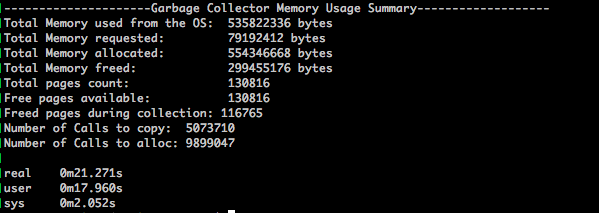
\includegraphics[width=\linewidth]{TicTacToeGC.png}
%   \end{minipage}

%   \textbf{Non-Gargage Collected}
%   \begin{minipage}{.49\textwidth}
%       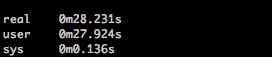
\includegraphics[width=\linewidth]{TicTacToeNoGC.png}
%   \end{minipage}
% \end{figure}


\subsection{Improving If Statements}
We decided to extend the WACC language with additional conditional branching statements; `if' statements without an `else' branch and `switch' statements. Initially to implement the `if' statements without an `else' branch we defined a new data type called `StmtIfNoElse' which had only the condition and the `then' branch associated with it but this added a lot of repetitive code as it was extremely similar to our `StmtIf'. To overcome this problem, we made use of Haskell's Maybe monad to  define `if' statements to have a Maybe block. We then had to change Parser.hs to allow this new syntax and then we had to add the new semantics to SemCheck.hs. The difference in semantic checking between an `if' statement with an `else' branch and one without was that in the case where the `else' block was empty we had to show that the `if' statement never necessarily returns a value.  Finally we had to ensure the correct assembly code was generated which meant changing CodeGen.hs to have a case expression to deal with if the block contained a value (Just b) or was empty (Nothing).
For `switch' statements we had to define new keywords in lexer.x for `switch' and `case'. Then, similarly we had to add switch statements to our semantic checker and parser and edit how the assembly code is generated.
\subsection{Type System improvements}
\subsubsection{Extending Pairs to Tuples}
One limited feature of WACC was the ability to deal with pairs instead of arbitrarily sized tuples. So a nice extension was to expand WACC to support tuples. The first step in this extension was to control the would-be redundancy if we kept all the code handling pairs and creating new code for tuples. So what was done was to naturally consider pairs as a subset of tuples. The only difference in code then would be on the lexer and the parser, but from the parser on we considered pairs as tuples and we only wrote code regarding tuples. The only problem then was accessing a pair with \texttt{fst} and \texttt{snd}. We made the decision that tuples were to be accesed in the same manner as arrays (i.e. \texttt{a[1]}), so then it  was an easy fix as we just considered \texttt{fst p = p[0]} and \texttt{snd p = p[1]}.

\begin{lstlisting}
begin
  int[] arr = [1,2,4,5];
  tuple(int, bool, char, int[]) tup = newtuple(1, false, 'c', arr);
  println tup[0]; # Prints 1.
  println tup[3][2] # Prints 4.
end
\end{lstlisting}

The second problem we encountered was that now arrays and tuples are accessed in the same manner. However, tuples can only be accesed with literal integers (so
then \texttt{int b = 2; println tup[b]} is ilegal but \texttt{int b = 2; println tup[2]} is legal in our extension) while arrays can be indexed with expressions. So we changed our design of arrays and merged the two into an IndexingElem instead of having TupleElem and ArrayElem. This helped solved the problem because now it was a matter of just pattern matching in the appropiate moment as we always carry around the type of the IndexingElem; either a tuple or an array.


\subsubsection{Structure Types}
We have extended the type system by adding both product (structs) and sum (tagged union) types.
These types work in a structural way, ie two type are equivalent is their members are the same,
rather whether their name matches.

Moreover a variable can be assigned any value which is a sub-type of the variable's type. A
sub-type is a type which exposes at least all of it's parent's behaviours. For example, for structs
a sub-type must have every field present in the parent, and of the same types, but may also have some more.

For example, in the following example, $p1$'s type is a subtype of $p2$'s, as both fields $x$ and
$y$ are present and have the correct type.

\begin{lstlisting}
{ int x, int y, int z } p1 = { x = 3, y = 4, z = 5 };
{ int x, int y } p2 = point;
\end{lstlisting}

Similarily, when calling a function, for each argument, any subtype of it may be given.
\begin{lstlisting}
void print_point({ int x, int y } p) is
  print "{ x = ", x, ", y = ", y, " }"
end

{ int x, int y, int z } p = { x = 3, y = 4, z = 5 };
call print_point(p);
\end{lstlisting}

Structures are implemented by attributing a distinct index to every possible field name. In the examples
above, $x$, $y$, and $z$ could for example be attributed indices 0, 1 and 2 respectively.
Note that the indices are shared by every struct in the program.

For every struct defined by the program, the compiler generates a virtual table, which map for each field
present in the structure the offset of that field with respect to the beggining of the structure.
A pointer to the vtable of the structure is placed at it's first word.

Field access happens as follows. First, the pointer to the vtable is loaded from the structure. The field's
index is known at compile time and is used to retrieve the offset from the vtable. Finally the offset is
added to the address of the struct, resulting in the address of the field.

\begin{lstlisting}
vtable = object[0]
offset = vtable[index]
data   = object[offset]
\end{lstlisting}

This makes field access more expensive than direct offsetting, as three memory accesses are required each time.
This is however a constant and moderate cost, as opposed to performing a map lookup, as dynamically typed languages.

While multiple optimisation could be added, we did not have time to implement them.
For example, the compiler could save the pointer to the vtable in a register between field accesses, reducing the
number of memory access to only 2. It could even save the offset itself if a single field is accessed multiple
times (in a loop for example), resulting in a single memory access. Additionally, in many cases, the compiler
has enough information the determine the structure's actual type, and compute the offsets at runtime

\subsubsection{Union Types}
Variable of union types may take any value of the types that compose it.
\begin{lstlisting}
(int|char) x = 5;
x = 'C';
(int|char|string) y = x;
y = "Hello";
\end{lstlisting}

In order to use the value, type switching must be used. Within each case block, the variable has the type that was
matched.
\begin{lstlisting}
void print_intOrCharOrString((int|char|string) x) is
  switch type(x)
  case int:
    print "x + 5 = ", x + 5
  case char:
    print "ord(x) = ", ord(x)
  case string:
    print "x = \"", x, "\""
  end
end
\end{lstlisting}

Union types are stored on the heap as two words. The first word is a tag, making it possible to determine the actual
type, while the second word stores the actual value, either directly for primitive types, or as a pointer.
For each type susceptible to be used in a union type, a unique tag is assigned, very much like indices for field members
are assigned.

When assigning a non-union value to a union variable, it gets automatically promoted by allocating the said structure.
When assigning a union value to a union variable, the same two word object is simply reused.

Type switching is done by comparing the tag in the union value with the one corresponding to the type we match to.
The value is then extracted, and made available inside the block.

While not normally a valid type, $null$ is allowed within union types. This permits nullable values for any type.
\begin{lstlisting}
void print_maybeInt((int|null) x) is
  switch type(x)
  case int:
    print "x = ", x
  case null:
    # Nothing useful can be done with x here
    print "x is null"
end
\end{lstlisting}

\subsubsection{Type synonyms}
With the new features, types can become long and cumbersome to type. To solve that, we've added type synonyms. Type synonyms
create exact aliases between a name and a type. The name is not used when checking type equality, only the structural typing
rules described above.

\begin{lstlisting}
type point = { int x, int y };
type maybePoint = (point | null);
type intOrChar = (int | char);
type intOrCharOrString = (intOrChar | string);
type threeInts = tuple(int, int, int);

void print_intOrChar(intOrChar x) is
  ...
end

let p : point = { x = 5, y = 6 };
\end{lstlisting}

Type synonyms may be used whereever a usual type would appear.
Types must be defined before they can be referenced. This ensures that recursive types cannot be created, as this would make
probably type equality checking equivalent to checking for graph isomorphism, and would make type checking much more complex.

\subsection{Foreign Function Interface}
While building more complex programs, the WACC language often turns up to be impractical or incapable of doing some tasks
(advanced IO for instance). Instead of adding features to the language every time, it may be useful to implement them in C
and exposing them to the WACC source. This may be done through the FFI.

\begin{lstlisting}
ffi void   srand(int);
ffi int    rand();
ffi string itoa(int) = wacc_itoa;

call srand(12345);
int r = call rand();
string random = call itoa(r);
\end{lstlisting}

The first name is the name of the function as used inside WACC program, while the second one is the symbol used to link,
typically the name of the C function. If not specified, the symbol name is the same as the function name.
Most predefined C functions cannot be used as is and must be wrapped using some custom binding, since other than primitive
types, WACC types do not have the same representation as usual C types.

The FFI also allows defining opaque types, which can be stored and passed around inside the WACC program, but not create nor
used directly. The may contain any one word value, typically a pointer to some complex data structure. The type checker
garantees that the value cannot be modified nor accessed other than through correctly-typed FFI calls.

\begin{lstlisting}
ffi type socket;

ffi socket connect(string)      = wacc_socket_connect;
ffi void   send(socket, string) = wacc_socket_send;
ffi void   close(socket)        = wacc_socket_close;

socket s = connect("www.example.org:1234");
send(s, "Hello World");
close(s);
\end{lstlisting}

\subsection{Concurrency}
We have added support for concurrency to WACC by using the $async$/$await$ pattern. This is inspired by the same
$async$/$await$ pattern available in C\#, or more recently in Python 3.5. Support for asynchronous network is
implemented on top of it, using Linux's epoll mechanism. Finally, channels, analogous to the ones present in Go,
have been added as well.

\subsubsection{Resumable functions}
As the first step torwards concurrency, resumable functions have been added to the WACC language.
Resumable functions run normally until they reach a wait point, in which case the local variables live at this point,
(liveness information produced by the register allocator is used at this effect) are saved to a block of memory allocated
on the heap, and yield by return a pointer to that block to their caller. When called again with this pointer as an argument,
they restore the local variables and resume from the wait point.
Such a function is declared as $async$.

The only possible wait point is an $await$ statement to another $async$ function. When reaching an $await$ statement,
the function is called as usual, but if the called functions yields, the state block it returned is saved along with the
other locals, and the current function yields as well, so will it's parent, and so on, unwinding the entire call stack.
When resumed, the current function calls the function again with it's saved state, waiting for it to produce a return value.
A function may yield multiple times before producing such value, and the call stack gets unwinded everytime.

In addition to returning it's state, when yielding, an $async$ function may also return an arbitrary value, which gets
returned by it's caller, and so. As such, the value gets propagated all the way down the call stack.

Alone this provides little benefit, since the only wait for an $async$ function to pause is by awaiting another $await$
function. However this becomes useful when combined with FFI functions. An FFI function can be declared as $async$ as well.
When called, it may yield a value which will be returned all the way down the call stack, until it reaches the initial
caller, typically some C runtime.

\subsubsection{Cooperative Scheduling}
The runtime keeps a list of tasks, essentially paused functions, and executes each until it yields. The yielded value
informs the runtime onto what should be done with the task. It may for example, remove the task from the ready list for
a certain amount time while running the other ready tasks in the meantime. This effectively allows for multiple tasks to
appear to be running simultaneously, where one runs while the others are paused.

It is important to note that this represents cooperative scheduling, which alleviates the usual problems arised by
concurrency. Indeed, a function may only pause while executing an $await$ statement. This means a function is guaranteed
that no other task will modify the heap between $await$ calls.

Finally, the $fire$ statement may be used to spawn a new task. It will perform the specified call to an $async$ function
within that new task, without waiting for it to complete. This is analogous to the $go$ statement from the Go language.

\subsubsection{Event loop and asynchronous networking}
The provided runtime maintains a list of ready tasks, along with a minimum heap of sleeping tasks, sorted by wakeup time.
It also uses Linux's epoll mechanism to be able to wait on arbitrary file descriptors.

Extra FFI functions are available in order to create sockets, returning opaque types as described earlier. All sockets
are marked as non blocking. Each socket also has two task list, for tasks trying to receive from and send to the socket.
$async$ FFI functions are used to send to and receive from sockets.

Taking the case of a read, if an attempt to read fails with an $EAGAIN$ error, ie no data is currently available, then
the function yields, while asking the runtime to add the current task to the socket's receive list. The socket's file
descriptor is added to the epoll structure. When the kernel notifies the runtime that data is available on that file
descriptor, all tasks on the socket's receive list are put back onto the ready list.

\begin{lstlisting}
ffi       socket server(int)          = wacc_socket_server;
ffi async socket accept(socket)       = wacc_socket_accept;
ffi async string recv(socket)         = wacc_socket_recv;
ffi async bool   send(socket, string) = wacc_socket_send;

async void handle(socket conn) do
  while true do
      let msg = call recv(conn);
      call send(conn, msg)
  done
end

socket s = call server(1234);
while true do
  let connection = call accept(s);
  fire handle(connection)
done
\end{lstlisting}

\subsubsection{Channels}
As the last concurrency feature, we have added channels, analogous to the ones present in Go.
Channels allow values to read and written to it. They are unbuffered, implying that writing to a channel will block
until another task reads from it. Channels are created using the $chan()$ right hand side, and using the $<-$ operator
to send and receive values.

\begin{lstlisting}
async void sender(chan(int)) is
  let x = 0;
  while true do
    ch <- x;
    x = x + 1
  end
end

async void receiver(chan(int) ch) is
  while true do
    let x = <- ch;
    println "x = ", x
  end
end

let ch : chan(int) = chan();
fire sender(ch);
fire receiver(ch);
\end{lstlisting}

Channels are implemented using FFI async functions, but require special language support as polymorphism is not generally
possible. As a consequence, channel operations must be done within $async$ functions.

In the runtime, channels are similar to sockets. Each channel has two task lists, for receiving and sending tasks.
The main difference with sockets is that no file descriptor is used. A receiving task is woken up when another task sends
a value, and vice-versa.

\section{Backwards Compatibility}
While implementing the various extensions, we have strived to keep backwards compatibility with the original WACC language,
as well as making the new features as integrated as possible. For instance, rather than having both pairs and arbitrary length
tuples, we've made one a superset of the other, and make it a single functionality, when keeping the previous syntax.

As a result, only two tests on fail on LabTS. The first one, $ifNoelse.wacc$, enforces an else block after an if, but this
is one of our extension, so this is the expected behaviour. The second one, $printAllTypes.wacc$, times out on LabTS but
produces the correct result when run locally. This is due to the optimised register allocation algorithm, which consumes a
lot of time when many local variables are live simultaneously.

\end{document}
